% Lecture file created by Gemini
% Class: Quantum Information With Atoms and Photons
% Professor: Pietro Silvi
% Date: 2025-10-16
\lecture{2}{Degenerate Perturbation Theory}{2025-10-16}

% --- Start writing here ---
\begin{enumerate}
  \setcounter{enumi}{3} 
  \item Perturbation Theory (the indefendent)\
done in a way that is useful\
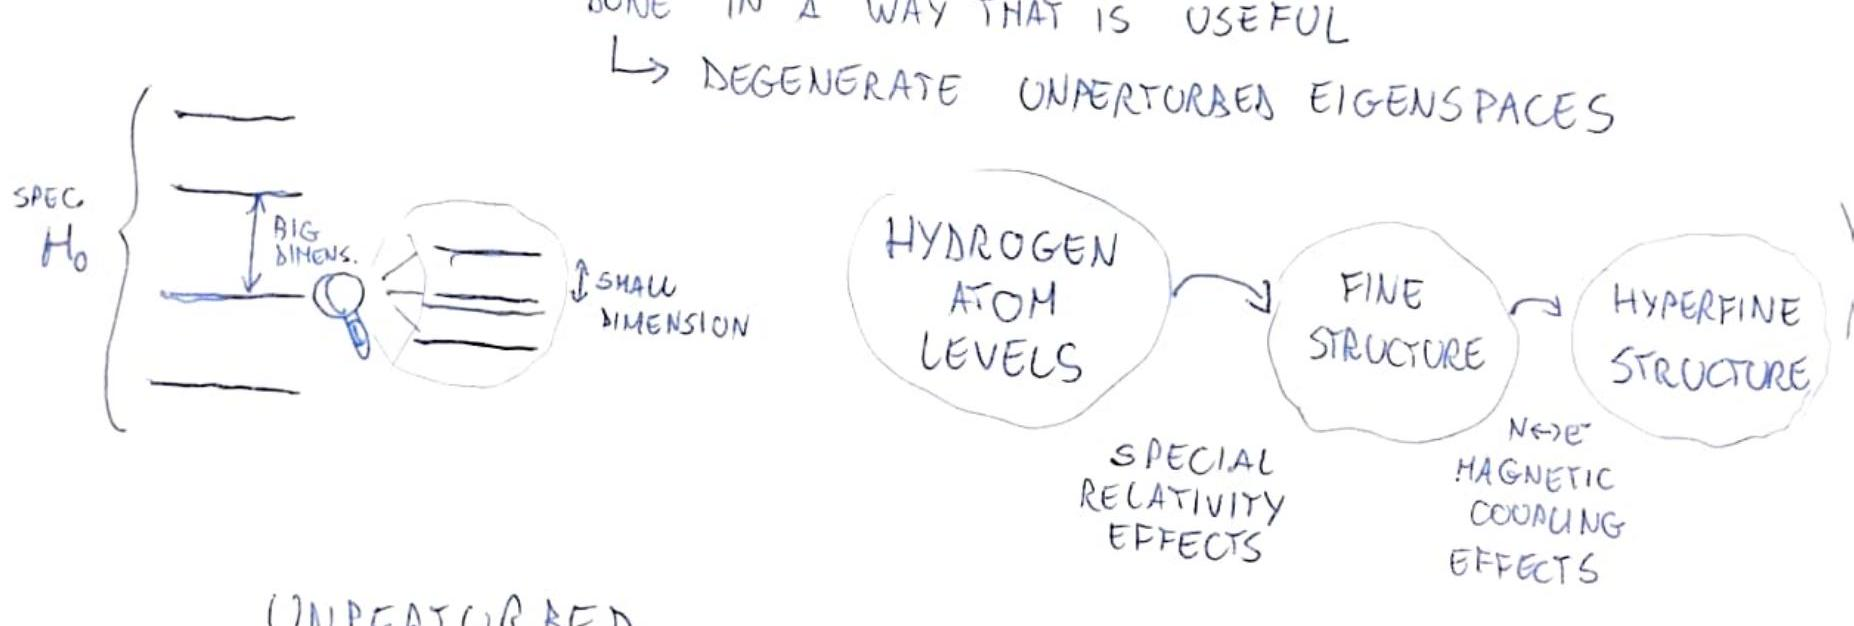
\includegraphics[max width=\textwidth, center]{2025_10_16_f6b2ddb567eefef2c7a2g-1(1)}
\end{enumerate}

UNPERTURBED

\section*{hamiltonian}
$H_{0}\left|\varepsilon^{(0)}, J\right\rangle=\varepsilon^{(0)}\left|\varepsilon^{(0)}, J\right\rangle$\
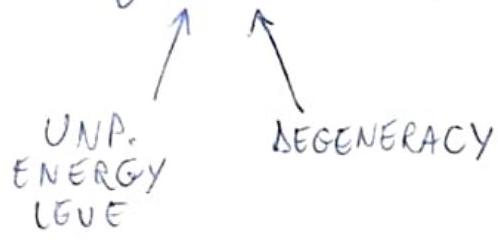
\includegraphics[max width=\textwidth, center]{2025_10_16_f6b2ddb567eefef2c7a2g-1}

EXAMPLE

$$
\left(\begin{array}{rll}
\varepsilon_{0} & & \\
& \varepsilon_{0} & \\
& & \rightarrow \\
& & \mid \varepsilon_{1}
\end{array}\right) \xrightarrow{\rightarrow}\left|\varepsilon_{0}, 1\right\rangle=\left(\begin{array}{l}
1 \\ 0 \\ 0
\end{array}\right)=\left(\begin{array}{l}
0 \\ 1 \\ 0
\end{array}\right)=\left(\begin{array}{l}
0 \\ 0 \\ 1
\end{array}\right)
$$

$\widetilde{\varepsilon}_{n}=\varepsilon_{n}^{(0)}+\lambda \varepsilon_{n}^{(1)}+\lambda^{2} \varepsilon_{n}^{(2)}+...$\
$\left|\tilde{\varepsilon}_{n}\right\rangle=\left|\varepsilon_{n}^{(0)}\right\rangle+\lambda\left|\varepsilon_{n}^{(1)}\right\rangle+\cdots$ Also WITH $J$
$\left(H_{0}+\lambda V\right)\left(\left|\varepsilon^{(0)}, J\right\rangle+\lambda\left|\varepsilon^{(1)}, J^{1}\right\rangle+\ldots\right)=\left(\varepsilon^{(0)}+\lambda \varepsilon^{(1)}+\ldots\right)\left(\left|\varepsilon^{(1)}, J\right\rangle+\lambda \mid \varepsilon^{(1)}, J\right.$\
ORDER $1=\lambda^{\circ}$\n$H_{0}\left|\varepsilon^{(0)}, J\right\rangle=\varepsilon^{(0)}\left|\varepsilon^{(0)}, J\right\rangle$ well, AT LEAST IT IS CONSISTENT

ORSER $\lambda=\lambda^{1}$\n$V\left|\varepsilon^{(0)}, J\right\rangle+H_{0}\left|\varepsilon^{(1)}, J^{\prime}\right\rangle=\varepsilon^{(1)}\left|\varepsilon^{(0)}, J\right\rangle+\varepsilon^{(0)}\left|\varepsilon^{(1)}, J^{\prime}\right\rangle$

$$
\Pi=\Pi^{+}=\Pi^{2}
$$

$\left.\begin{array}{l}\text { I now DEFINE THE PROSECYOR } \\ \text { ONTO THE } \varepsilon^{(0)} \text { EIGENSPACE OF } H_{0}\end{array}\right\} \quad \Pi_{\varepsilon_{0}}=\sum_{\zeta}\left|\varepsilon^{(0)}, J\right\rangle\left\langle\varepsilon^{(0)}, J\right|$

$$
\prod_{\varepsilon_{0}} H_{0}=H \prod_{0}=\varepsilon^{(0)} \Pi \quad \ldots \text { AND I HULTIPLY LEFT. } 
$$

$\Pi_{\varepsilon_{0}} V\left|\varepsilon^{(0)}, J\right\rangle+\underbrace{\ldots}_{\varepsilon_{0}} H\left|\varepsilon^{(1)}, J^{\prime}\right\rangle=\varepsilon^{(1)} \Pi_{\varepsilon_{0}}\left|\varepsilon^{(0)}, J\right\rangle+\varepsilon^{(0)} \Pi_{\varepsilon_{0}}\left|\varepsilon^{(0)}, J^{\prime}\right\rangle$

$$
\varepsilon^{(0)} \Pi_{\varepsilon^{(0)}}\left|\varepsilon^{(+)}, J^{\prime}\right\rangle
$$

$\left|\varepsilon^{(0)}, J\right\rangle=\pi_{\varepsilon^{(0)}}\left|\varepsilon^{(0)}, J\right\rangle$

$$
\prod_{\varepsilon(0)}\left|\varepsilon^{(0)}, j\right\rangle=\left|\varepsilon^{(0)}, j\right\rangle
$$

$$
(\underbrace{\Pi_{\varepsilon_{0}} \vee \Pi_{\varepsilon_{0}}})\left|\varepsilon^{(0)}, J\right\rangle=\varepsilon^{(1)}\left|\varepsilon^{(0)}, J\right\rangle \quad \forall J
$$

$\Rightarrow \underbrace{(\pi V \pi)^{+}=\pi^{+} V^{+} \pi^{+}=\pi V \pi}_{\text {HERMITIAN }}$\nEigenvalue Equation
$\rightarrow$ IT TEUS US HOW THE SEGENERACY IS REMOVES AND\nHOW THE RESOLVED STATES LOOK LIKE
Notice $\rightarrow$ the resolves states are (NOT) a correction from an arbitrary $|\varepsilon, j\rangle$ (see example later)

EXCERCISE
$\lambda H_{\varepsilon_{i}^{(1)}}^{(1)}\left|\varepsilon^{(0)}, J\right\rangle=\lambda \varepsilon^{(1)}\left|\varepsilon^{(0)}, J\right\rangle$
where $\lambda M_{\varepsilon_{0}}^{(1)}=\lambda\left(\Pi_{\varepsilon^{(0)}} \vee \Pi_{\varepsilon^{(0)}}\right)$

CONTRACT * WITH

$$
\left\langle\varepsilon_{n}^{(0)}, J\right| \text { AND }
$$
LEARN SOMETHING ABOUT $\left|\varepsilon^{(1)}, J\right\rangle$

GA HIGHER ORDERS OF DEG-REMOVING HAMICTONIANS $L$ USUALLY THE COWEST NONZERO ORDER COUNTS

NON-DEG

$$
\begin{aligned}
& H_{0}^{(1)}=\Pi_{\varepsilon_{0}} V \Pi_{\varepsilon_{0}} \\
& \varepsilon^{(1)}=\left\langle\varepsilon_{0}\right| V\left|\varepsilon_{0}\right\rangle \\
& H_{\varepsilon_{0}}^{(2)}=\Pi_{\varepsilon_{0}} \vee R_{\varepsilon_{0}} \vee \Pi_{\varepsilon_{0}} \\
& \Leftrightarrow \varepsilon^{(2)}=\sum_{\varepsilon_{n} \neq \varepsilon_{0}} \frac{\left|\left\langle\varepsilon_{n}\right| V\left|\varepsilon_{0}\right\rangle\right|^{2}}{\varepsilon_{n}^{(0)}-\varepsilon_{n}^{(0)}} \\
& =\left\langle\varepsilon_{0}\right| V \underbrace{\left(\sum_{\varepsilon_{n} \varepsilon_{0}} \frac{\left|\varepsilon_{n} \times \varepsilon_{n}\right|}{\varepsilon_{0}^{(0)}-\varepsilon_{n}^{(0)}}\right)}_{\text {MOORE-PENROSE }} V\left|\varepsilon_{0}\right\rangle \\
& \text { PSEUDOINVERSE } \\
& \text { (INVERY ONCY THE) } \\
& \downarrow \\
& R_{\varepsilon_{0}}=\left(\begin{array}{ccl}
0 & & \\
& \frac{1}{\varepsilon_{0}-\varepsilon_{1}} & \\
& & \frac{1}{\varepsilon_{0}-\varepsilon_{i}}
\end{array}\right) \\
& A=\left(\begin{array}{lll}0 & & \\ & 1 & \\ & & 2\end{array}\right) \quad A^{\prime \prime \prime}=\left(\begin{array}{lll}0 & & \\ & 1 & \\ & & 1 / 2\end{array}\right) \\
& \varepsilon^{(2)}=\left\langle\varepsilon_{0}\right| V\left(\varepsilon_{0}^{(0)} \mathbb{1}-H_{0}\right)^{-1} V \mid \varepsilon \\
& H_{\varepsilon_{0}}^{(3)}=\Pi_{\varepsilon_{0}} V R_{\varepsilon_{0}} V R_{\varepsilon_{0}} V \Pi_{\varepsilon_{0}}-\Pi_{\varepsilon_{0}} V \Pi_{\varepsilon_{0}} V R_{\varepsilon_{0}}^{2} V \Pi_{\varepsilon_{0}} \\
& H_{\varepsilon_{0}}^{(4)}=\Pi_{\varepsilon_{0}} V R_{\varepsilon_{0}} V R_{\varepsilon_{0}} V R_{\varepsilon_{0}} V \Pi_{\varepsilon_{0}}-\Pi_{\varepsilon_{0}} V R_{\varepsilon_{0}}^{2} V \Pi_{\varepsilon_{0}} V R_{\varepsilon_{0}} V \Pi_{\varepsilon_{0}} \\
& -\pi \vee \pi \vee R \vee R^{2} \vee \pi-\pi \vee \pi \vee R^{2} \vee R V \pi \\
& +\pi V \pi V \pi V R^{3} V \pi
\end{aligned}
$$

(5) nonsense

EXERCISE THE LAMBDA SYSTEM (USEEVI FOR

$$
\frac{\hbar}{|0\rangle} \frac{|e\rangle}{|1\rangle}
$$

$$
|0\rangle=\left(\begin{array}{l}
1 \\ 0 \\ 0
\end{array}\right) \quad |e\rangle=\left(\begin{array}{l}
0 \\ 1 \\ 0
\end{array}\right) \quad |1\rangle=\left(\begin{array}{l}
0 \\ 0 \\ 1
\end{array}\right)
$$

$$
H_{0}=\left(\begin{array}{ccc}
0 & & \\ & +\Delta & \\ & & 0
\end{array}\right)
$$

$$
V=\left(\begin{array}{ccc}
0 & \Omega & \\ \Omega & 0 & \Omega \\ & \Omega & 0
\end{array}\right)=\Omega\left(\begin{array}{ll}1 & 1 \\ 1 & 1\end{array}\right)
$$

UN PERTURBED
GAMILTONIAN

$$
\left.\left.\begin{array}{lll}\Pi_{0}=\left(\begin{array}{ll}1 & \\ 0 & 1 \\ & 1\end{array}\right) & R_{0}=\left(\begin{array}{cc}0 & \\ -\frac{1}{\Delta} & \\ & \\ \Pi_{\Delta}=\left(\begin{array}{ll}0 & \\ 1\end{array}\right) & \end{array}\right. & H_{0}^{(1)}=0 \\ & 0
\end{array}\right)\left(\begin{array}{cc}\frac{1}{\Delta} & \\ & 0 \\ & \\ & +\frac{1}{\Delta}\end{array}\right)\right)\left(H_{\Delta}^{(1)}=0
$$

$H_{0}^{(2)}=\Pi_{0} \vee R_{0} \vee \Pi_{0}=\frac{\Omega^{2}}{\Delta}\left(\begin{array}{ll}1 & 0 \\ 1 & 1
\end{array}\right)\left(\begin{array}{ll}0 & 1 \\ 1 & 1 \\ 1 & 0
\end{array}\right)\left(\begin{array}{ll}0 & \\ 1 & 0
\end{array}\right)\left(\begin{array}{ll}1 & 1 \\ 1 & 1\end{array}\right)\left(\begin{array}{ll}1 & \\ 0 & 1
\end{array}\right)=$

$$
\Delta\left(t+\frac{2 \Omega^{2}}{\Delta^{2}}\right)=-\frac{\Omega^{2}}{\Delta}\left(\begin{array}{ll}1 & 1 \\ 1 & 0 \\ 1 & 1\end{array}\right)
$$

\begin{center}
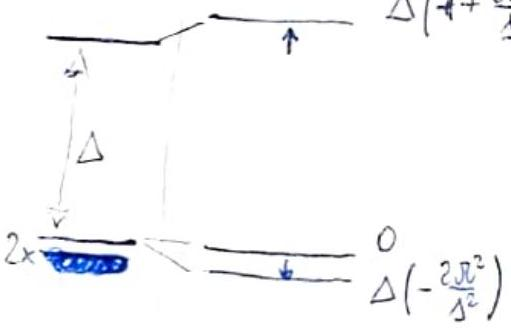
\includegraphics[width=0.5\textwidth]{2025_10_16_f6b2ddb567eefef2c7a2g-4}
\end{center}

$$
\begin{aligned}
& \text { DARH } \\
& \text { STAT } \\
& \left.\frac{2 \Omega^{2}}{\Delta}\right)
\end{aligned}
$$

$$
\begin{aligned}
& \frac{|0\rangle+|1\rangle}{\sqrt{2}} \leadsto \varepsilon^{(2)}=-\frac{2 \Omega^{2}}{\Delta} \\
& \frac{|0\rangle-|1\rangle}{\sqrt{2}} \leadsto \varepsilon^{(2)}=0 \text { DARK }
\end{aligned}
$$

$H_{2}^{(2)}=\ldots .=|e \times e|\left(+\frac{2 \Omega^{2}}{\Delta}\right) \quad \varepsilon_{e}^{(0)}+\varepsilon_{e}^{(2)}=\Delta+\frac{2 \Omega^{2}}{\Delta}$\n11)\
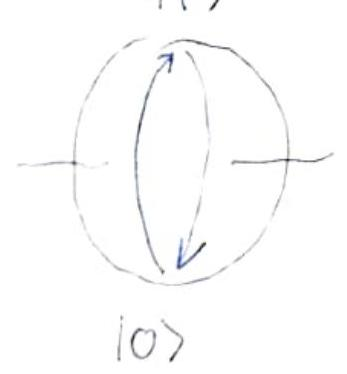
\includegraphics[width=0.5\textwidth, center]{2025_10_16_f6b2ddb567eefef2c7a2g-4(1)}

\section*{FUL RABI}
$$
=\Delta\left(1+\frac{2 \Omega^{2}}{\Delta^{2}}\right)
$$

frequency $\left|\left(0-\frac{2 \Omega^{2}}{\Delta}\right)\right|=\frac{2 \Omega^{2}}{\Delta}=\Delta\left(\frac{2 \Omega^{2}}{\Delta^{2}}\right) \ll \Delta$
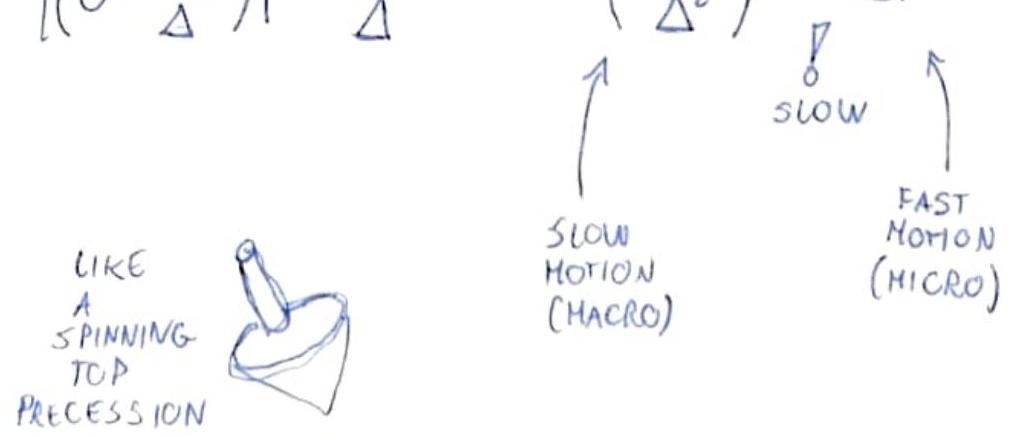
\includegraphics[width=0.5\textwidth, center]{2025_10_16_f6b2ddb567eefef2c7a2g-4(2)}

\section*{SAME Problem BUT (NO) PERTURBATION tHEORY}
$\hbar=1$

$$
\begin{array}{ll}
H_{0}=\left(\begin{array}{ccc}
0 & & \\ & +\Delta & \\ & & 0
\end{array}\right) \quad V=\left(\begin{array}{ccc}
0 & \Omega & \\ \Omega & 0 & \Omega \\ & \Omega & 0
\end{array}\right) & \text { EXACT } \\ H_{\text {TOT }}=H_{0}+V=\Delta\left(\begin{array}{ccc}
0 & \eta & \\ \eta & 1 & \eta \\ & \eta & 0
\end{array}\right) \quad \text { WITH } \quad \eta=\frac{\Omega}{\Delta} & \text { SHALU } \\ \text { PARAMETER } 
\end{array}
$$

$\left|\begin{array}{ccc}-\lambda & \eta & \\ \eta & 1-\lambda & \eta \\ & \eta & -\lambda\end{array}\right|=P(\lambda)=\lambda^{2}(1-\lambda)+2 \lambda \eta^{2}=-\lambda\left(\lambda^{2}-\lambda-2 \eta^{2}\right)$

$$
P(\lambda)=0 \rightarrow \lambda=\frac{1}{2}\left(1 \pm \sqrt{1+8 \eta^{2}}
$$

$P(\lambda)=0 \rightarrow \lambda={ }_{0}$\n$\Delta \sim \frac{1}{\uparrow} \Delta\left(\frac{1}{2}+\frac{1}{2} \sqrt{1+8 \frac{\Omega^{2}}{\Delta^{2}}}\right) \geqslant \Delta\left(\frac{1}{2}+\frac{1}{2}\left(1+4 \frac{\Omega^{2}}{\Delta^{2}}\right)\right)$\n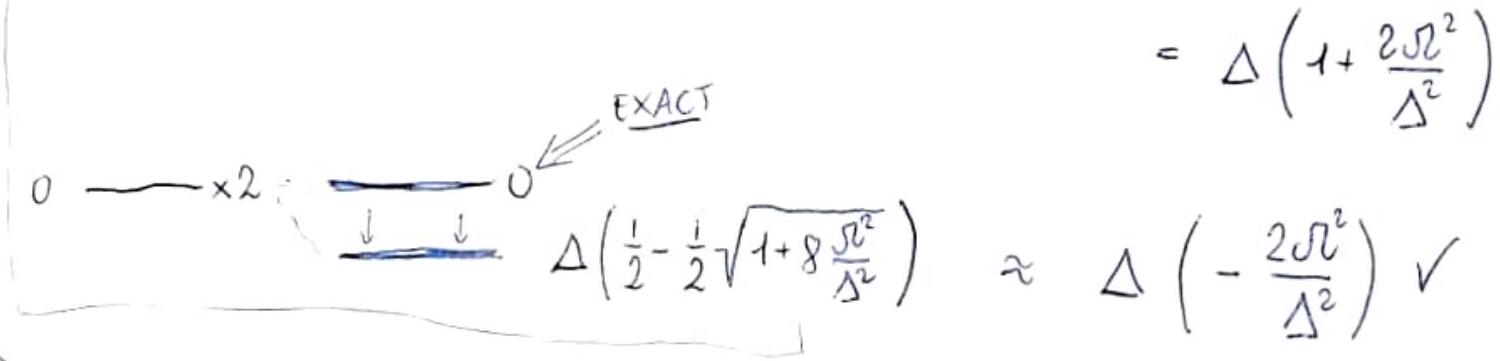
\includegraphics[width=0.5\textwidth, center]{2025_10_16_f6b2ddb567eefef2c7a2g-5(1)}\
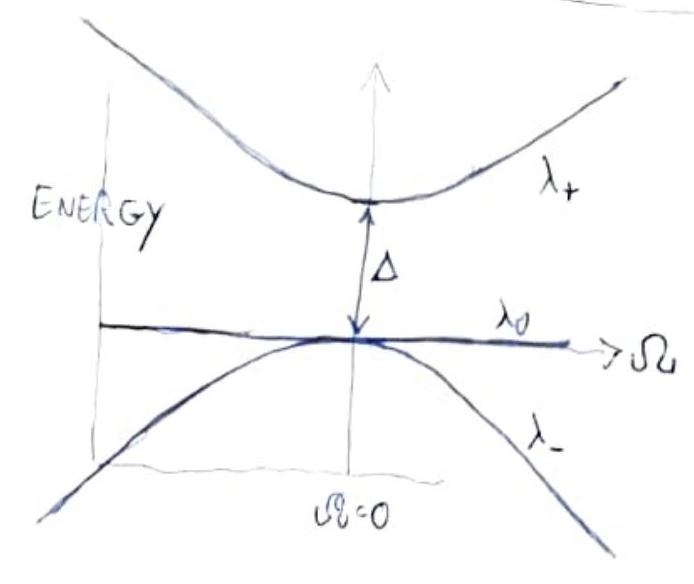
\includegraphics[width=0.5\textwidth, center]{2025_10_16_f6b2ddb567eefef2c7a2g-5}

Secular Motion

Microhotion $\mu^{\mu^{m} \eta_{\eta}}$\nsee marco's lecture
$\sim$ LIKE $A$ RABI $\sigma^{*}$\
$|0\rangle{ }^{\curvearrowleft}|1\rangle$
EREQUENCY $\left|0-\frac{2 \Omega^{2}}{\Delta}\right|=\frac{2 \Omega^{2}}{\Delta}$\nDERIOD $\frac{\pi \Delta}{\Omega^{2}}$ (slow)
WIGGLES OF AOPULATION OF $|e\rangle$

FREQUENCY $\sim \Delta$
PERIOD $\frac{2 \pi}{\Delta}$ (FAST)
5. Time-Orderes Exponential

$$
\begin{aligned}
&i \frac{d}{d t}|\psi(t)\rangle =H(t)|\psi(t)\rangle \\
&i \frac{d}{d t} U\left(t, t_{0}\right)|\psi \phi_{0}\rangle =H(t) U\left(t, t_{0}\right)|\psi_{0}\rangle
\end{aligned}
$$

$|\psi(t)\rangle=U\left(t, t_{0}\right)|\psi_{0}\rangle \quad$ WITH

$$
\underset{\substack{\text { ASSITIVITY } \ U\left(t_{2}, t_{1}
ight) \cup\left(t_{1}, t_{0}
ight)}}{=U\left(t_{2}, t_{0}
ight)}
$$

$$
U(t, t)=\mathbb{1} \quad \begin{gathered}\text { Ideourity } \\ \text { CONNETION }\end{gathered}
$$

SHAU DREHENT $\rangle \delta t \leadsto \quad U(t+\delta t, \underbrace{\left.t_{0}\right)}_{\text {TAYCOR }}=U\left(t, t_{0}\right)+\delta t \frac{d U}{d t}\left(t, t_{0}\right)+\theta\left(\delta t^{2}\right)$

$$
\begin{gathered}
U(t+\delta t) U\left(t, t_{0}\right)=U\left(t+\delta t, t_{0}\right)=(1-i \delta H(t)) U\left(t, t_{0}\right)+\theta\left(\delta t^{2}\right) \\
U(t+\delta t, t) \approx \exp (-i H(t) \delta t)+\theta\left(\delta t^{2}\right)
\end{gathered}
$$

$t_{0} \quad$ sivide in $N$ wifelenals $t>t_{0}$

$$
\delta t=\frac{t-t_{0}}{N}
$$

$U\left(t, t_{0}\right)=U(t, t-\delta t) \frac{U(t-\delta t, t-2 \delta t) \cdots C}{\text { THE ORSER is THPORTANT}}\left(t_{0}+\delta t, t_{0}\right)$

$$
=\exp (-i \delta t H(t-\delta t)) \exp (-i \delta t H(t-2 \delta t)) \cdots \exp (-i \delta t H(t))+\theta
$$

$$
U\left(t, t_{0}\right)=\lim _{\delta t \rightarrow 0}\left(\sum_{\text {EXPRESSION }}^{T H 1 S}(V)=\operatorname{Iexp}\left(-i \int_{t_{0}}^{t} H\left(t^{\prime}\right) d t^{\prime}\right)
ight.
$$

(or $N \rightarrow \infty$)\
THE HISTORICAL REASON WHY IT IS factoral! WRITMEN LIKE THIS IS DUE TO THE\nAlso-ReE $\downarrow{ }_{t}$ DYSON SERIES\
$U\left(t, t_{0}\right)=1+\sum_{n=1}^{\infty}(-2)^{n} \int_{t_{0}}^{t} d t_{1} \int_{t_{0}}^{t_{1}} d t_{2} \ldots \int_{t_{0}}^{t_{n}-t_{n}} d t_{n} H\left(t_{1}\right) H\left(t_{2}\right) \ldots H\left(t_{n}\right)
